\documentclass[a4paper,10pt,twoside,final,spanish]{article}

% Preámbulo - Parte A

\usepackage[utf8]{inputenc} % Soporte para los acentos
\usepackage[T1]{fontenc}

\usepackage[spanish]{babel} % Capítulos, seciones, etc. en español

\usepackage[margin=2cm]{geometry} % Diseño del documento

\usepackage{multicol} % Escribir doble columna

\usepackage{xcolor} % Usar colores
\usepackage{pstricks}

\usepackage{enumerate} % Cambiar etiquetas de numeración
\usepackage[shortlabels]{enumitem} % Manejo adicional de etiquetas de numeración

\usepackage{graphicx} % Manejo de gráficos y figuras

\usepackage{makeidx} % Índice alfabético

% Paquetes adicionales de símbolos matemáticos
\usepackage{amsmath,amssymb,amsfonts,latexsym} 

% \usepackage{pslatex} % Fuente Times
% \usepackage{mathpazo} % Fuente Palatino
% \usepackage{mathptmx} % Fuente Times
% \usepackage{bookman} % Fuente Bookman
\usepackage{newcent} % Fuente New Century Schoolbook
% \usepackage{helvet} % Fuente Helvetica
% \usepackage{palatino} % Fuente Palatino
% \usepackage{pxfonts} % Fuente 
% \usepackage{txfonts} % Fuente
% \usepackage{concrete} % Fuente
% \usepackage{cmbright} % Fuente
% \usepackage{fourier} % Fuente

\usepackage{booktabs} % Opciones adicionales para el entorno tabular
\usepackage{longtable} % Para tablas de más de una página

\usepackage{tikz} % Creación de gráficos

\usepackage{hyperref}

\usepackage{textcomp}
\usepackage{gensymb} %para los grados celcius
\usepackage[makeroom]{cancel} %Para tachar expresiones matemáticas
\newcommand\Ccancel[2][black]{\renewcommand\CancelColor{\color{#1}}\cancel{#2}}

\usepackage{soul} % para tachar texto
\pagestyle{headings}
% Para encerrar expresiones con círculos
\usepackage{mathtools}% superior to amsmath
\usepackage{siunitx} % para escribir grados minutos segundos
\usepackage{tikz}
\makeatletter
\newcommand\mathcircled[1]{%
  \mathpalette\@mathcircled{#1}%
}
\newcommand\@mathcircled[2]{%
  \tikz[baseline=(math.base)] \node[draw,circle,inner sep=1pt] (math) {$\m@th#1#2$};%
}
\makeatother
%---
\usepackage{fancyhdr} %Para usar encabezados y pies personalizados
	\pagestyle{fancy}
	\fancyhf{}
	\fancyhead[LE,RO]{Mecánica del Continuo}
	\fancyhead[RE,LO]{Campos de Velocidad y Condiciones de Compatibilidad}
	\fancyfoot[LE,RO]{\thepage}
	\fancyfoot[RE,LO]{Darién Julián Ramírez}	
	\renewcommand{\footrulewidth}{1pt}
%---
\usepackage{listings} %Para escribir códigos
\lstset{language=XML,
	basicstyle=\footnotesize,
	numbers=left,
 	stepnumber=1,
	numbersep=8pt,
	showspaces=false,               % show spaces adding particular underscores
  	showstringspaces=false,         % underline spaces within strings
  	frame=lines,                   % adds a frame around the code
	tabsize=4,                      
  	captionpos=b,                   % sets the caption-position to bottom
  	breaklines=true,                % sets automatic line breaking
}
%---

% Preámbulo - Parte B

\title{\Huge Mecánica del Continuo \\
			 Trabajo Práctico Nº6  \\
			 Campos de Velocidad y Condiciones de Compatibilidad}
\author{Darién Julián Ramírez}
\date{}

% Cuerpo del documento

\begin{document}

\maketitle % Mostrar título

\section*{Ejercicio 1}

Considere el movimiento de un fluido con componentes de velocidad $u$ y $v$ derivadas de un potencial $\Phi$:
   
\[
\begin{array}{cc}
\displaystyle u=\frac{\partial\Phi}{\partial x}, &
\displaystyle v=\frac{\partial\Phi}{\partial y}
\end{array}
\]

mientras que la componente $w$ es idénticamente cero. Dibuje los campos de velocidad 
para los potenciales siguientes:

\begin{enumerate}[a)]
\item $\displaystyle \Phi=\frac{1}{4\pi}\log(x^{2}+y^{2})=\frac{1}{2\pi}\log r;
\quad r^{2}=x^{2}+y^{2}$
\item $\displaystyle \Phi=x$
\item $\displaystyle \Phi=Ar^{n}\cos(n\theta);
\quad \theta=\tan^{-1}\left(\frac{y}{x}\right)$
\item $\displaystyle \Phi=\frac{\cos\theta}{r}$
\end{enumerate}

Se recomienda presentar los resultados utilizando software como Matlab® u Octave(GNU). 

\begin{figure}[htbp]
\begin{minipage}{0.5\linewidth}

\textbf{Nota:} Un flujo de un campo cuyas componentes de velocidad se obtienen de una función potencial $\Phi(x,y,z)$ es llamado \textit{flujo potencial}. En los ejemplos mencionados en este problema tenemos varios casos en los cuales $\Phi$ se expresa en términos de coordenadas polares $r,\theta$. Si notamos que el vector velocidad $(u,v)$  es exactamente el gradiente de una función escalar $\Phi(x,y,z)$, vemos por análisis  vectorial que las componentes de velocidad en coordenadas polares son:

\[
\begin{array}{cc}
\displaystyle u_{r}=\frac{\partial\Phi(r,\theta)}{\partial r}, &
\displaystyle u_{\theta}=\frac{1}{r}\frac{\partial\Phi(r,\theta)}{\partial\theta}
\end{array}
\]

\end{minipage} \hfill \begin{minipage}{0.45\linewidth}

\centerline{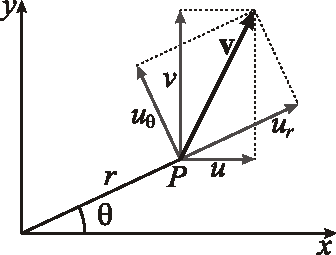
\includegraphics{ej1}}
\caption{Relación entre condenadas cartesianas y polares.}
\label{fig:ej1}

\end{minipage}
\end{figure}

donde $u_{r},u_{\theta}$ son las componentes de velocidad en las direcciones radial y tangencial, respectivamente. Quedan relacionadas con las componentes en coordenadas Cartesianas de esta forma:

\[
u_{r}=\frac{\partial\Phi(r,\theta)}{\partial r}
=\frac{\partial\Phi}{\partial x}\frac{\partial x}{\partial r}
+\frac{\partial\Phi}{\partial y}\frac{\partial y}{\partial r}
=u\cos\theta+v\sin\theta
\]

\[
u_{\theta}=\frac{1}{r}\frac{\partial\Phi(r,\theta)}{\partial\theta}
=\frac{1}{r}\left(
\frac{\partial\Phi}{\partial x}\frac{\partial x}{\partial\theta}
+\frac{\partial\Phi}{\partial y}\frac{\partial y}{\partial\theta}
\right)
=-u\sin\theta+v\cos\theta
\]

\dotfill

\begin{quote}
\begin{enumerate}[a)]

\item

\begin{minipage}{0.5\linewidth}

\begin{align*}
u &= \frac{1}{2\pi}\frac{x}{x^{2}+y^{2}} \\
v &= \frac{1}{2\pi}\frac{y}{x^{2}+y^{2}}
\end{align*}

\end{minipage} \hfill \begin{minipage}{0.5\linewidth}

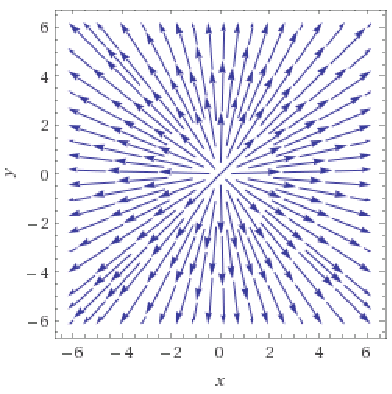
\includegraphics{ej1a}

\end{minipage}

\item

\begin{minipage}{0.5\linewidth}

\begin{align*}
u &= 1 \\
v &= 0
\end{align*}

\end{minipage} \hfill \begin{minipage}{0.5\linewidth}

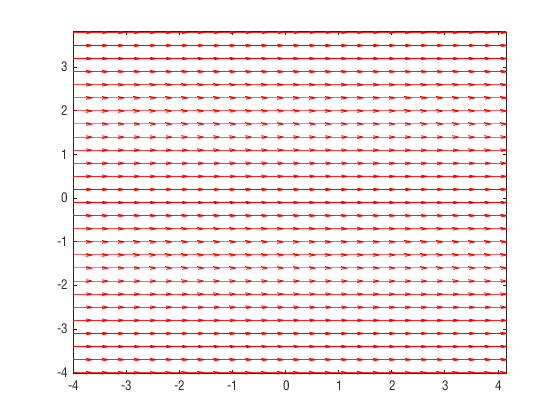
\includegraphics[width=\linewidth]{ej1b}

\end{minipage}

\item

\begin{minipage}{0.5\linewidth}

\begin{align*}
u &= 2An\cos{(n\theta)}(x^{2}+y^{2})^{n-1}x \\
v &= 2An\cos{(n\theta)}(x^{2}+y^{2})^{n-1}y
\end{align*}

\end{minipage} \hfill \begin{minipage}{0.5\linewidth}

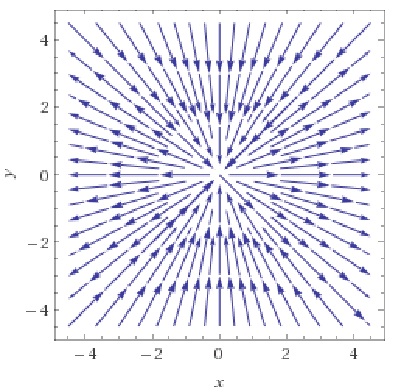
\includegraphics[width=\linewidth]{ej1c}

\end{minipage}

\item

\begin{minipage}{0.5\linewidth}

\begin{align*}
u &= -\frac{x\cos{\theta}}{(x^{2}+y^{2})^{\frac{3}{2}}} \\
v &= -\frac{y\cos{\theta}}{(x^{2}+y^{2})^{\frac{3}{2}}}
\end{align*}

\end{minipage} \hfill \begin{minipage}{0.5\linewidth}

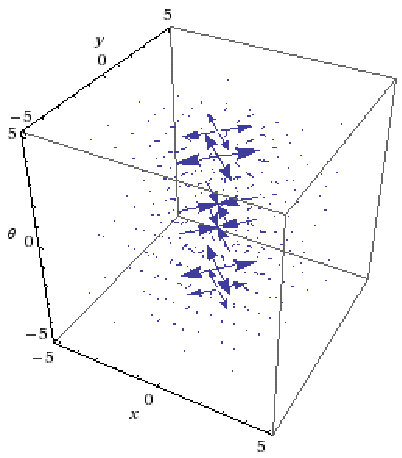
\includegraphics[width=\linewidth]{ej1d}

\end{minipage}

\end{enumerate}
\end{quote}

\section*{Ejercicio 2}

El movimiento de un fluido incompresible en dos dimensiones puede obtenerse de una \textit{función de corriente} $\Psi$ del siguiente modo:

\[
u=-\frac{\partial\Psi}{\partial y}; \quad
v=\frac{\partial\Psi}{\partial x};  \quad
w=0
\]

Esquematice las líneas de corriente $\Psi=cte$ para las siguientes funciones y compare 
los resultados con los del problema anterior:

\begin{enumerate}[a)]
\item $\Psi=c\theta$
\item $\Psi=y$
\item $\Psi=Ar^{n}\sin(n\theta)$
\item $\displaystyle \Psi=-\frac{\sin\theta}{r}$
\end{enumerate}

Superponga las gráficas de estas funciones con su correspondiente campo del ejercicio 1.

\dotfill

\begin{quote}
\begin{enumerate}[a)]

\item

\begin{minipage}{0.5\linewidth}

\begin{align*}
u &= 0 \\
v &= 0
\end{align*}

\end{minipage} \hfill \begin{minipage}{0.5\linewidth}

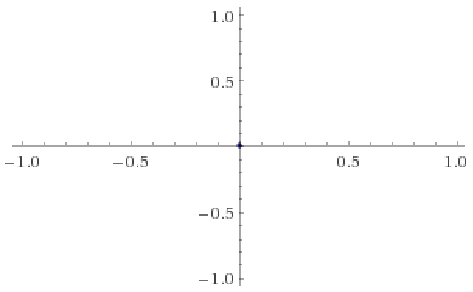
\includegraphics{ej2a}

\end{minipage}

\item

\begin{minipage}{0.5\linewidth}

\begin{align*}
u &= -1 \\
v &= 0
\end{align*}

\end{minipage} \hfill \begin{minipage}{0.5\linewidth}

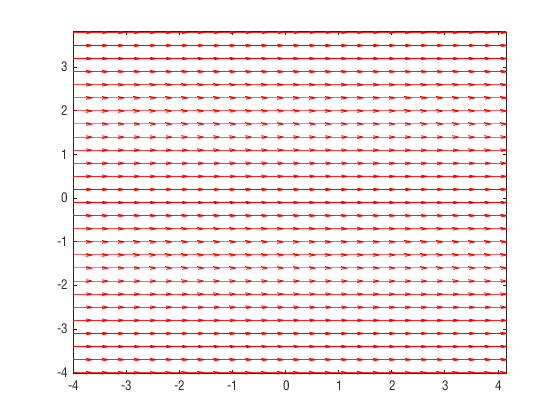
\includegraphics[width=\linewidth]{ej1b}

\end{minipage}

\item

\begin{minipage}{0.5\linewidth}

\begin{align*}
u &= 2An\sin{(n\theta)}(x^{2}+y^{2})^{n-1}x \\
v &= 2An\sin{(n\theta)}(x^{2}+y^{2})^{n-1}y
\end{align*}

\end{minipage} \hfill \begin{minipage}{0.5\linewidth}

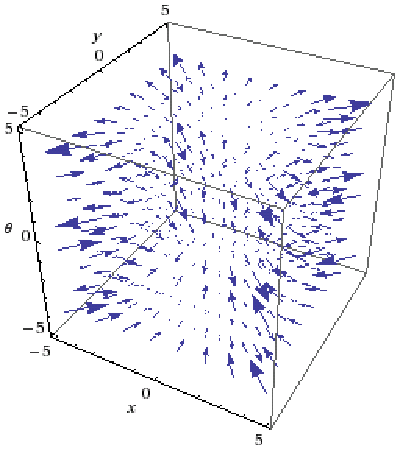
\includegraphics[width=\linewidth]{ej2c}

\end{minipage}

\item

\begin{minipage}{0.5\linewidth}

\begin{align*}
u &= \frac{x\sin\theta}{(x^{2}+y^{2})^{\frac{3}{2}}} \\
v &= \frac{y\sin\theta}{(x^{2}+y^{2})^{\frac{3}{2}}}
\end{align*}

\end{minipage} \hfill \begin{minipage}{0.5\linewidth}

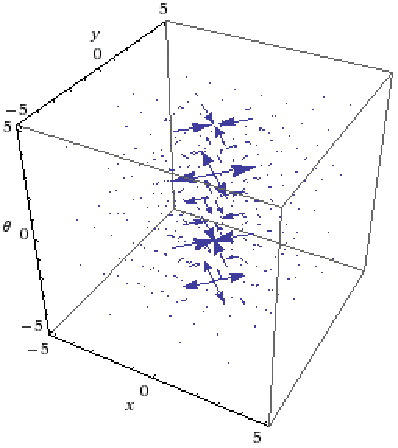
\includegraphics[width=\linewidth]{ej2d}

\end{minipage}

\end{enumerate}
\end{quote}

\section*{Ejercicio 3}

Para los flujos descritos por los potenciales listados en el ejercicio de arriba:

\begin{enumerate}[a)]
\item Muestre que la vorticidad desaparece en cada caso. 
\item Obtenga las expresiones para el tensor tasa de deformación. 
\end{enumerate}

\dotfill

\begin{quote}
\begin{enumerate}[a)]
\item \textit{Tensor de vorticidad:}

\begin{align*}
\Omega_{ij} &= \frac{1}{2}\left(\frac{\partial v_{j}}{\partial x_{i}}
- \frac{\partial v_{i}}{\partial x_{j}}\right)
\end{align*}
	
	\begin{enumerate}[$\Psi$a.]
	\item
	\begin{align*}
	\Omega_{ij} &= \frac{1}{2}\left(\frac{\partial v}{\partial x}
	-\frac{\partial u}{\partial y}\right)
	=\frac{1}{2}(0-0)=0
	\end{align*}
	
	\item
	\begin{align*}
	\Omega_{ij} &= \frac{1}{2}\left(\frac{\partial v}{\partial x}
	-\frac{\partial u}{\partial y}\right)
	=\frac{1}{2}(0-0)=0
	\end{align*}
	
	\item 
	\begin{align*}
	\Omega_{ij} &= \frac{1}{2}\left(\frac{\partial v}{\partial x}
	-\frac{\partial u}{\partial y}\right) \\
	&= \frac{1}{2}\left(4A(n-1)nxy\sin{(n\theta)}(x^{2}+y^{2})^{n-2}
	-4A(n-1)nxy\sin{(n\theta)}(x^{2}+y^{2})^{n-2}\right) \\
	&= \frac{1}{2}\cdot 0 \\
	&= 0
	\end{align*}
	
	\item
	\begin{align*}
	\Omega_{ij} &= \frac{1}{2}\left(\frac{\partial v}{\partial x}
	-\frac{\partial u}{\partial y}\right) \\
	&= \frac{1}{2}\left(-\frac{3xy\sin{\theta}}{(x^{2}+y^{2})^{\frac{5}{2}}}
	+\frac{3xy\sin{\theta}}{(x^{2}+y^{2})^{\frac{5}{2}}}\right) \\
	&= \frac{1}{2}\cdot 0 \\
	&= 0
	\end{align*}
	\end{enumerate}

\item \textit{Tensor tasa de deformación:}

\begin{align*}
V_{ij} &= \frac{1}{2}\left(\frac{\partial v_{i}}{\partial x_{j}}
+ \frac{\partial v_{j}}{\partial x_{i}}\right)
=\frac{1}{2}\left(\frac{\partial u}{\partial y}
+ \frac{\partial v}{\partial x}\right)
\end{align*}

	\begin{enumerate}[$\Psi$a.]
	\item 
	\begin{align*}
	V_{ij} &= \frac{1}{2}(0+0)=0
	\end{align*}
	
	\item 
	\begin{align*}
	V_{ij} &= \frac{1}{2}(0+0)=0
	\end{align*}
	
	\item 
	\begin{align*}
	V_{ij} &= \frac{1}{2}\left(4A(n-1)nxy\sin{(n\theta)}(x^{2}+y^{2})^{n-2}
	+4A(n-1)nxy\sin{(n\theta)}(x^{2}+y^{2})^{n-2}\right) \\
	&= 4A(n-1)nxy\sin{(n\theta)}(x^{2}+y^{2})^{n-2}
	\end{align*}
	
	\item
	\begin{align*}
	V_{ij} &= \frac{1}{2}\left(-\frac{3xy\sin{\theta}}{(x^{2}+y^{2})^{\frac{5}{2}}}
	-\frac{3xy\sin{\theta}}{(x^{2}+y^{2})^{\frac{5}{2}}}\right) \\
	&= -\frac{3xy\sin{\theta}}{(x^{2}+y^{2})^{\frac{5}{2}}}
	\end{align*}
	\end{enumerate}

\end{enumerate}

\end{quote}

\section*{Ejercicio 4}

Suponga que se nos da el siguiente campo de desplazamiento definido en un círculo unitario:

\[
\begin{array}{l}
u=ax^{2}+bxy+c \\
v=by^{2}+cx+mz \\
w=mz^{3}
\end{array}
\] 
 
¿Existe compatibilidad? 

\dotfill

\begin{quote}
\textit{Ecuaciones de compatibilidad en tres dimensiones:}

\begin{align*}
\frac{\partial^{2}e_{xx}}{\partial y \partial z}
&= \frac{\partial}{\partial x}\left(
-\frac{\partial e_{yz}}{\partial x}
+\frac{\partial e_{zx}}{\partial y}
+\frac{\partial e_{xy}}{\partial z}\right) \\
\frac{\partial^{2}e_{yy}}{\partial z \partial x}
&= \frac{\partial}{\partial y}\left(
-\frac{\partial e_{zx}}{\partial y}
+\frac{\partial e_{xy}}{\partial z}
+\frac{\partial e_{yz}}{\partial x}\right) \\
\frac{\partial^{2}e_{zz}}{\partial x \partial y}
&= \frac{\partial}{\partial z}\left(
-\frac{\partial e_{xy}}{\partial z}
+\frac{\partial e_{yz}}{\partial x}
+\frac{\partial e_{zx}}{\partial y}\right) \\
2\frac{\partial^{2}e_{xy}}{\partial x \partial y}
&= \frac{\partial^{2}e_{xx}}{\partial y^{2}}
+\frac{\partial^{2}e_{yy}}{\partial x^{2}} \\
2\frac{\partial^{2}e_{yz}}{\partial y \partial z}
&= \frac{\partial^{2}e_{yy}}{\partial z^{2}}
+\frac{\partial^{2}e_{zz}}{\partial y^{2}} \\
2\frac{\partial^{2}e_{zx}}{\partial z \partial x}
&= \frac{\partial^{2}e_{zz}}{\partial x^{2}}
+\frac{\partial^{2}e_{xx}}{\partial z^{2}} \\
\end{align*}

Se ha verificado utilizando cálculo simbólico.

\end{quote}

\section*{Ejercicio 5}

Suponga que el campo de desplazamiento en un círculo unitario es:
 
\[
\begin{array}{l}
u=ar\log\theta       \\
v=ar^{2}+c\sin\theta \\
w=0
\end{array}
\] 

\begin{enumerate}[a)]
\item ¿El campo es compatible?
\item Grafique el campo de desplazamientos e interprete los resultados.
\end{enumerate}

\textbf{Ayuda:} Convertir el campo de desplazamientos a coordenadas polares y luego utilizar la siguiente condición de compatibilidad:

\centerline{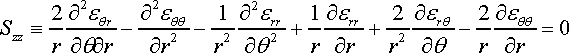
\includegraphics{ej5}}

También puede verificar esta ecuación de compatibilidad utilizando sofware simbólico (Maple®, Mathematica®, Matlab®, Octave(GNU) ó Maxima(GNU)). 

\dotfill

\begin{quote}
Como el campo es continuo y diferenciable, verifica compatibilidad. Como el $\ln{\theta}$ en $u$ posee discontinuidades en $\theta=0$, no es un campo de desplazamientos válido.

$u$ y $v$ dependen de $r$ y $\theta$ pero generan sus componentes proyectadas en ejes cartesianos.

Se restringe el problema físico a $0<\theta\leq 2\pi$ y se evita la discontinuidad en cero y la doble asignación de desplazamientos para $\theta\leq 2\pi$.
\end{quote}

\section*{Ejercicio 6}

Rotación infinitesimal y vorticidad. Sean, $u(x)$ $v(x)$ campos de desplazamiento y velocidad, respectivamente. Definimos el \textit{tensor de spin} o de \textit{rotación infinitesimal} como:

\[
\omega_{ij}=\frac{1}{2}
\left(
\frac{\partial u_{j}}{\partial x_{i}}-\frac{\partial u_{i}}{\partial x_{j}}
\right)
\]
 
Para este tensor, construimos un vector dual (vector de rotación):

\begin{equation}
\omega_{k}=\frac{1}{2}\varepsilon_{kij}\omega_{ij} \implies
\omega_{ij}=\varepsilon_{ijk}\omega_{k}
\label{eq:eq1}
\end{equation}

Por otra parte, definimos el tensor de vorticidad como:

\[
\Omega_{ij}=\frac{1}{2}
\left(
\frac{\partial v_{j}}{\partial x_{i}}-\frac{\partial v_{i}}{\partial x_{j}}
\right)
\]
 
Para este tensor, construimos un vector dual (vector de vorticidad) con una convención 
ligeramente distinta a la anterior:
 
\begin{equation}
\Omega_{k}=\varepsilon_{kij}\Omega_{ij} \implies
\Omega_{ij}=\frac{1}{2}\varepsilon_{ijk}\Omega_{k}
\label{eq:eq2}
\end{equation}
 
(Notar que esta definición está cambiada en la tercera edición de Fung respecto de la 
segunda edición).

\begin{enumerate}[a.]
\item Demostrar que el vector de rotación o de spin puede interpretarse físicamente 
como la rotación que sufre el entorno del punto considerado.

\begin{quote}
\begin{align*}
du_{i} &= \frac{\partial u_{i}}{\partial x_{j}}dx_{j} & \\
&= \frac{1}{2}\frac{\partial u_{i}}{\partial x_{j}}dx_{j}
+\frac{1}{2}\frac{\partial u_{i}}{\partial x_{j}}dx_{j} & \\
&= {\blue \frac{1}{2}\frac{\partial u_{i}}{\partial x_{j}}dx_{j}}
{\red +\frac{1}{2}\frac{\partial u_{i}}{\partial x_{j}}dx_{j}}
{\blue +\frac{1}{2}\frac{\partial u_{j}}{\partial x_{i}}dx_{j}}
{\red -\frac{1}{2}\frac{\partial u_{j}}{\partial x_{i}}dx_{j}} & \\
&= {\red \frac{1}{2}\left(\frac{\partial u_{i}}{\partial x_{j}}
-\frac{\partial u_{j}}{\partial x_{i}}\right)}dx_{j}
{\blue +\frac{1}{2}\left(\frac{\partial u_{j}}{\partial x_{i}}
+\frac{\partial u_{i}}{\partial x_{j}}\right)}dx_{j} & \\
&= {\red -\omega_{ij}}dx_{j}{\blue +e_{ij}}dx_{j} & e_{ij} &= 0 \\
&= -\omega_{ij}dx_{j} & \omega_{ij} &= \varepsilon_{ijk}\omega_{k}\\
&= -\varepsilon_{ijk}\omega_{k}dx_{j} & \\
&= \varepsilon_{ikj}\omega_{k}dx_{j} & \\
&= (\mathbf{\omega}\times\mathbf{dx})_{i} & \\
\end{align*}
\end{quote}

\item Demostrar la relación que da el tensor de rotación en función de su vector dual 
(Ecuación: \ref{eq:eq1}).

\begin{quote}

Demostrar que $\omega_{ij}=\varepsilon_{ijk}\omega_{k}$ donde $\omega_{k}=\frac{1}{2}\varepsilon_{kij}\omega_{ij}$.

\begin{align*}
\omega_{ij} &= \varepsilon_{ijk}\omega_{k} 
& \textit{Por definición de vector de rotación infinitesimal.} \\
&= \varepsilon_{ijk}\frac{1}{2}\varepsilon_{kem}\omega_{em} 
& \textit{Reordenando.} \\
&= \frac{1}{2}\varepsilon_{ijk}\varepsilon_{kem}\omega_{em} 
& \textit{Permutando el primer épsilon.} \\
&= \frac{1}{2}\varepsilon_{kij}\varepsilon_{kem}\omega_{em} 
& \textit{Identidad épsilon-delta.} \\
&= \frac{1}{2}(\delta_{ie}\delta_{jm}-\delta_{im}\delta_{je})\omega_{em} 
& \textit{Distribuyendo.} \\
&= \frac{1}{2}(\delta_{ie}\delta_{jm}\omega_{em}-\delta_{im}\delta_{je}\omega_{em}) 
& \textit{Contrayendo índices.} \\
&= \frac{1}{2}(\delta_{ie}\omega_{ej}-\delta_{im}\omega_{jm})
& \textit{Contrayendo índices.} \\
&= \frac{1}{2}(\omega_{ij}-\omega_{ji})
& \textit{Antisimetría del tensor de rotación infinitesimal.} \\
&= \frac{1}{2}(\omega_{ij}+\omega_{ij})
& \textit{Sumando.} \\
&= \frac{1}{2}2\omega_{ij}
& \textit{Simplificando.} \\
&= \omega_{ij} \\
\end{align*}
\end{quote}

\item Demostrar la relación que da el tensor de vorticidad en función de su vector dual (Ecuación \ref{eq:eq2}).

\begin{quote}

Demostrar que $\Omega_{ij}=\frac{1}{2}\varepsilon_{ijk}\Omega_{k}$ donde $\Omega_{k}=\varepsilon_{kij}\Omega_{ij}$.

\begin{align*}
\Omega_{ij} &= \frac{1}{2}\varepsilon_{ijk}\Omega_{k} 
& \textit{Por definición de vector de vorticidad.} \\
&= \frac{1}{2}\varepsilon_{ijk}\varepsilon_{kem}\Omega_{em} 
& \textit{Permutando el primer épsilon.} \\
&= \frac{1}{2}\varepsilon_{kij}\varepsilon_{kem}\Omega_{em} 
& \textit{Identidad épsilon-delta.} \\
&= \frac{1}{2}(\delta_{ie}\delta_{jm}-\delta_{im}\delta_{je})\Omega_{em} 
& \textit{Distribuyendo.} \\
&= \frac{1}{2}(\delta_{ie}\delta_{jm}\Omega_{em}-\delta_{im}\delta_{je}\Omega_{em}) 
& \textit{Contrayendo índices.} \\
&= \frac{1}{2}(\delta_{ie}\Omega_{ej}-\delta_{im}\Omega_{jm})
& \textit{Contrayendo índices.} \\
&= \frac{1}{2}(\Omega_{ij}-\Omega_{ji})
& \textit{Antisimetría del tensor vorticidad.} \\
&= \frac{1}{2}(\Omega_{ij}+\Omega_{ij})
& \textit{Sumando.} \\
&= \frac{1}{2}2\Omega_{ij}
& \textit{Simplificando.} \\
&= \Omega_{ij} \\
\end{align*}
\end{quote}

\item Demostrar que: $\mathbf{\Omega}=\mathbf{rot}(\mathbf{v})$

\begin{align*}
\textbf{rot}(\mathbf{v}) &= \nabla\times\mathbf{v} \\
&= \varepsilon_{ijk}\frac{\partial v_{k}}{\partial x_{j}} \\
&= \varepsilon_{ijk}\left(
{\blue \frac{1}{2}\frac{\partial v_{k}}{\partial x_{j}}}
{\red +\frac{1}{2}\frac{\partial v_{k}}{\partial x_{j}}}
{\blue +\frac{1}{2}\frac{\partial v_{j}}{\partial x_{k}}}
{\red -\frac{1}{2}\frac{\partial v_{j}}{\partial x_{k}}}\right) \\
&= \varepsilon_{ijk}{\red \frac{1}{2}\left(
\frac{\partial v_{k}}{\partial x_{j}}
-\frac{\partial v_{j}}{\partial x_{k}}\right)}
+\varepsilon_{ijk}{\blue \frac{1}{2}\left(
\frac{\partial v_{k}}{\partial x_{j}}
+\frac{\partial v_{j}}{\partial x_{k}}\right)} \\
&= \varepsilon_{ijk}{\red \Omega_{jk}}+\frac{1}{2}\left(
\varepsilon_{ijk}\frac{\partial v_{k}}{\partial x_{j}}
+\varepsilon_{ijk}\frac{\partial v_{j}}{\partial x_{k}}\right) \\
&= \varepsilon_{ijk}\Omega_{jk}+\frac{1}{2}\left(
\varepsilon_{ijk}\frac{\partial v_{k}}{\partial x_{j}}
+\varepsilon_{ikj}\frac{\partial v_{k}}{\partial x_{j}}\right) \\
&= \varepsilon_{ijk}\Omega_{jk}+\frac{1}{2}\left(
\varepsilon_{ijk}\frac{\partial v_{k}}{\partial x_{j}}
-\varepsilon_{ijk}\frac{\partial v_{k}}{\partial x_{j}}\right) \\
&= \varepsilon_{ijk}\Omega_{jk}+\frac{1}{2}\cdot 0 \\
&= \varepsilon_{ijk}\Omega_{jk} \\
&= \Omega_{i} \\
&= \mathbf{\Omega} \\
\end{align*}

\item Dar la interpretación física del vector vorticidad.

\begin{quote}
\begin{align*}
dv_{i} &= \frac{\partial v_{i}}{\partial x_{j}}dx_{j} & \\
&= \frac{1}{2}\frac{\partial v_{i}}{\partial x_{j}}dx_{j}
+\frac{1}{2}\frac{\partial v_{i}}{\partial v_{j}}dx_{j} & \\
&= {\blue \frac{1}{2}\frac{\partial v_{i}}{\partial x_{j}}dx_{j}}
{\red +\frac{1}{2}\frac{\partial v_{i}}{\partial x_{j}}dx_{j}}
{\blue +\frac{1}{2}\frac{\partial v_{j}}{\partial x_{i}}dx_{j}}
{\red -\frac{1}{2}\frac{\partial v_{j}}{\partial x_{i}}dx_{j}} & \\
&= {\red \frac{1}{2}\left(\frac{\partial v_{i}}{\partial x_{j}}
-\frac{\partial v_{j}}{\partial x_{i}}\right)}dx_{j}
{\blue +\frac{1}{2}\left(\frac{\partial v_{j}}{\partial x_{i}}
+\frac{\partial v_{i}}{\partial x_{j}}\right)}dx_{j} & \\
&= {\red -\Omega_{ij}}dx_{j}{\blue +V_{ij}}dx_{j} & V_{ij} &= 0 \\
&= -\Omega_{ij}dx_{j} & \Omega_{ij} &= \frac{1}{2}\varepsilon_{ijk}\Omega_{k}\\
&= -\frac{1}{2}\varepsilon_{ijk}\Omega_{k}dx_{j} & \\
&= \frac{1}{2}\varepsilon_{ikj}\Omega_{k}dx_{j} & \\
&= \frac{1}{2}(\mathbf{\Omega}\times\mathbf{dx})_{i} & \\
\end{align*}
\end{quote}
\end{enumerate}

\section*{Apéndice}

\textit{Tensor tasa de deformación (simétrico):}

\begin{align*}
V_{ij} &= \frac{1}{2}\left(\frac{\partial v_{i}}{\partial x_{j}}
+ \frac{\partial v_{j}}{\partial x_{i}}\right)=V_{ji}
\end{align*}

\vspace{1em}

\textit{Tensor de vorticidad (antisimétrico):}

\begin{align*}
\Omega_{ij} &= \frac{1}{2}\left(\frac{\partial v_{j}}{\partial x_{i}}
- \frac{\partial v_{i}}{\partial x_{j}}\right)=-\Omega_{ji}
\end{align*}

\vspace{1em}

\textit{Gradiente de velocidad (matriz - tensor de rango 2):}

\begin{align*}
\nabla v &= \frac{\partial v_{i}}{\partial x_{j}} \\
&= \text{Tensor tasa de deformación}-\text{Tensor de vorticidad} \\
&= V_{ij}-\Omega_{ij} \\
&= \frac{1}{2}\left(\frac{\partial v_{i}}{\partial x_{j}}
+ \frac{\partial v_{j}}{\partial x_{i}}\right)
- \frac{1}{2}\left(\frac{\partial v_{j}}{\partial x_{i}}
- \frac{\partial v_{i}}{\partial x_{j}}\right)
\end{align*}

\vspace{1em}

\textit{Vector de vorticidad:}

\begin{align*}
\Omega_{k} &= \varepsilon_{kij}\Omega_{ij} & \implies &
&\Omega_{ij} &= \frac{1}{2}\varepsilon_{ijk}\Omega_{k}
\end{align*}

\vspace{1em}

\textit{Comparativa entre \textbf{rotación infinitesimal} y \textbf{vorticidad}:}

\begin{center}
\begin{tabular}{c | c | c} \toprule
       & Rotación infinitesimal & Vorticidad \\ \midrule
Tensor & $\displaystyle \omega_{ij}
=\frac{1}{2}\left(\frac{\partial u_{j}}{\partial x_{i}}
-\frac{\partial u_{i}}{\partial x_{j}}\right)
=\varepsilon_{ijk}\omega_{k}$ & $\displaystyle\Omega_{ij}
=\frac{1}{2}\left(\frac{\partial v_{j}}{\partial x_{i}}
- \frac{\partial v_{i}}{\partial x_{j}}\right)
=\frac{1}{2}\varepsilon_{ijk}\Omega_{k}$ \\
Vector & $\displaystyle\omega_{k}=\frac{1}{2}\varepsilon_{kij}\omega_{ij}$ & $\displaystyle\Omega_{k}=\varepsilon_{kij}\Omega_{ij}$ \\ \bottomrule
\end{tabular}
\end{center}

\vspace{1em}

\textit{Comparativa entre \textbf{deformación infinitesimal}, \textbf{rotación infinitesimal}, \textbf{tasa de deformación} y \textbf{vorticidad}:} \\

\begin{center}
\begin{tabular}{l c} \toprule
Deformación infinitesimal & $\displaystyle e_{ij}=\frac{1}{2}\left(\frac{\partial u_{j}}{\partial x_{i}}+\frac{\partial u_{i}}{\partial x_{j}}\right)$ \\ \midrule
Rotación infinitesimal    & $\displaystyle \omega_{ij}=\frac{1}{2}\left(\frac{\partial u_{j}}{\partial x_{i}}-\frac{\partial u_{i}}{\partial x_{j}}\right)$ \\ \midrule
Tasa de deformación       & $\displaystyle V_{ij}=\frac{1}{2}\left(\frac{\partial v_{i}}{\partial x_{j}}+\frac{\partial v_{j}}{\partial x_{i}}\right)$ \\ \midrule
Vorticidad                & $\displaystyle \Omega_{ij}=\frac{1}{2}\left(\frac{\partial v_{j}}{\partial x_{i}}- \frac{\partial v_{i}}{\partial x_{j}}\right)$\\ \bottomrule
\end{tabular}
\end{center}

\vspace{1em}

\textit{Ecuación de compatibilidad para el estado plano de tensiones:}

\begin{align*}
\frac{\partial^{2}e_{xx}}{\partial y^{2}}+\frac{\partial^{2}e_{yy}}{\partial x^{2}}
&= 2\frac{\partial^{2}e_{xy}}{\partial x \partial y}
\end{align*}

\vspace{1em}

\textit{Ecuaciones de compatibilidad en tres dimensiones:}

\begin{align*}
\frac{\partial^{2}e_{xx}}{\partial y \partial z}
&= \frac{\partial}{\partial x}\left(
-\frac{\partial e_{yz}}{\partial x}
+\frac{\partial e_{zx}}{\partial y}
+\frac{\partial e_{xy}}{\partial z}\right) \\
\frac{\partial^{2}e_{yy}}{\partial z \partial x}
&= \frac{\partial}{\partial y}\left(
-\frac{\partial e_{zx}}{\partial y}
+\frac{\partial e_{xy}}{\partial z}
+\frac{\partial e_{yz}}{\partial x}\right) \\
\frac{\partial^{2}e_{zz}}{\partial x \partial y}
&= \frac{\partial}{\partial z}\left(
-\frac{\partial e_{xy}}{\partial z}
+\frac{\partial e_{yz}}{\partial x}
+\frac{\partial e_{zx}}{\partial y}\right) \\
2\frac{\partial^{2}e_{xy}}{\partial x \partial y}
&= \frac{\partial^{2}e_{xx}}{\partial y^{2}}
+\frac{\partial^{2}e_{yy}}{\partial x^{2}} \\
2\frac{\partial^{2}e_{yz}}{\partial y \partial z}
&= \frac{\partial^{2}e_{yy}}{\partial z^{2}}
+\frac{\partial^{2}e_{zz}}{\partial y^{2}} \\
2\frac{\partial^{2}e_{zx}}{\partial z \partial x}
&= \frac{\partial^{2}e_{zz}}{\partial x^{2}}
+\frac{\partial^{2}e_{xx}}{\partial z^{2}} \\
\end{align*}

\begin{thebibliography}{99}
\bibitem{MCF}
Y. C. Fung,
\emph{A First Course in Continuum Mechanics}, 
tercera edición,
PRENTICE HALL,
1994.

\bibitem{IMCM}
Lawrence E. Malvern,
\emph{Introduction to the Mechanics of a Continuous Medium},
Prentice Hall,
1969. 
\end{thebibliography}

\end{document}